\section{Gesture Recognition}
Above sections described the necessary tools that are implemented to execute a real time hand gesture recognition system. In this thesis we have decided to train the system with static gestures. However, the system can be easily extended to recognize temporal gestures with the flexibility of Gesture Recognition Toolkit (GRT). Initially a set of simple gestures are chosen and the training data is collected for all those gestures.

\subsection{Hand Gestures Modeling}
In this thesis we have modeled five static hand gestures involving both the hands of the user. These are communicative hand gestures and they symbolize few referential action. Apart from Sign Language used by people with speech disability, various hand gestures are being used by humans in their day to day living. Figure \ref{fg:ges:signal} shows the hand signals used by different personnels in wide variety of application.

\begin{figure}
	[h] \centering 
	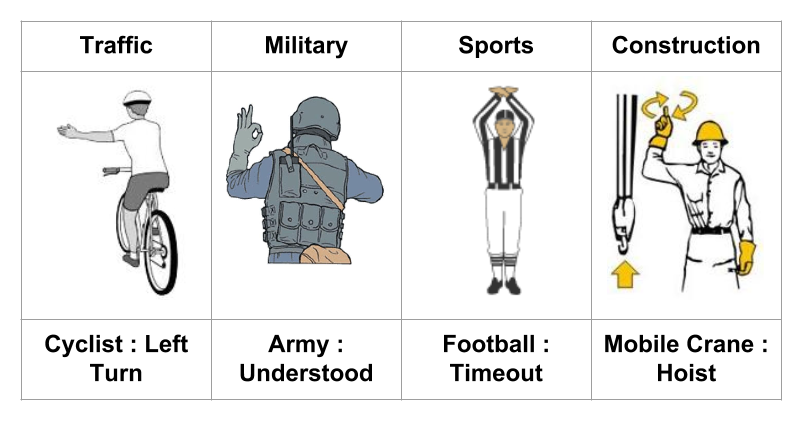
\includegraphics[height=7cm]{figures/content/ges-signals.png} \caption{Hand Signals} \label{fg:ges:signal} 
\end{figure}


This thesis focuses on hand gesture recognition to felicitate Human-Robot interactions. One greater application using hand gestures for robots is commanding the robot to move to another position. Additionally it could translate the gestures to spoken words to help people with speech disability.   

\begin{figure}
	\centering 
	\begin{minipage}
		{.45 
		\textwidth} \centering 
		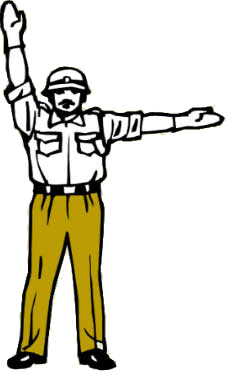
\includegraphics[height=7cm]{figures/content/ges-turn-left.jpg} \caption{Turn Left Gesture} \label{fg:ges:2} 
	\end{minipage}
	\begin{minipage}
		{.45 
		\textwidth} \centering 
		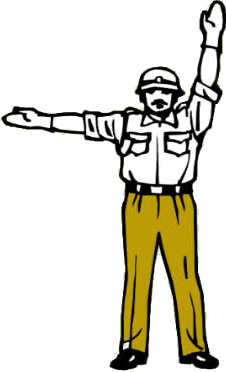
\includegraphics[height=7cm]{figures/content/ges-turn-right.jpg} \caption{Turn Right Gesture} \label{fg:ges:3} 
	\end{minipage}
	\begin{minipage}
		{.45 
		\textwidth} \centering 
		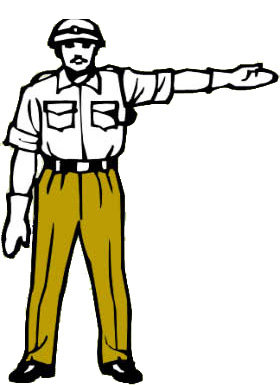
\includegraphics[height=7cm]{figures/content/ges-move-left.jpg} \caption{Move Left Gesture} \label{fg:ges:4} 
	\end{minipage}
	\begin{minipage}
		{.45 
		\textwidth} \centering 
		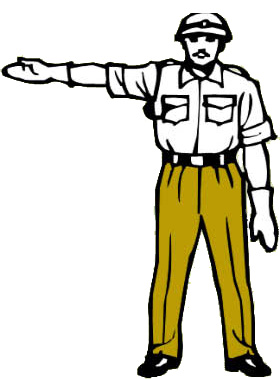
\includegraphics[height=7cm]{figures/content/ges-move-right.jpg} \caption{Move Right Gesture} \label{fg:ges:5} 
	\end{minipage}
	\begin{minipage}
		{.45 
		\textwidth} \centering 
		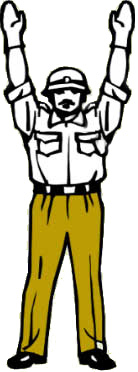
\includegraphics[height=7cm]{figures/content/ges-walk.jpg} \caption{Walk Gesture} \label{fg:ges:1} 
	\end{minipage}	
\end{figure}
\label{fg:ges:hands} 


Therefore, we have chosen five simple static gestures as shown in the figure \ref{fg:ges:hands} which are conceptualized by the traffic police hand signals. All the gestures are modeled to the direction of the user and they will be understood as mirrored gestures. For example, left side of the user will be right side to the robot that is facing the user. Additionally our system makes use of two dynamic gestures of NiTE which are used as focus gestures to gain control or start hand tracking.

\paragraph*{Turn Left} It is gesticulated as shown in the figure \ref{fg:ges:2} by holding the right hand up and left hand wide open. It refers to an action that turn to left and stay in position. 

\paragraph*{Turn Right} It is gesticulated as shown in the figure \ref{fg:ges:3} by holding the left hand up and right hand wide open. It refers to an action that turn to right and stay in position. 

\paragraph*{Move Left} It is gesticulated as shown in the figure \ref{fg:ges:4} by holding the right hand down and left hand wide open. It refers to an action that turn to left and keep moving in the forward direction.

\paragraph*{Move Right} It is gesticulated as shown in the figure \ref{fg:ges:4} by holding the left hand down and right hand wide open. It refers to an action that turn to right and keep moving in the forward direction.

\paragraph*{Walk} It is gesticulated as shown in the figure \ref{fg:ges:4} by holding the left and right hand up. It refers to an action that keep moving in the forward direction.

\paragraph*{Wave} It is gesticulated by holding a hand up and move it several times from left to right and back. This gesture is executed to initiate hand tracking, if no hands are tracked or tracked hand is been lost.

\paragraph*{Click} It is gesticulated by holding a hand up, push the hand towards the sensor then immediately pull the hand backwards. 

\subsection{Training} 
Our gesture recognition pipeline is configured to have 15 seconds preparation time and 20 seconds recording time with 6 dimensional input of both left and right hands at positions x, y and z in the Cartesian coordinates. Depth camera is at the origin of the coordinate system as shown in the figure \ref{fg:xtion:origin}.

\begin{figure}
	[h] \centering 
	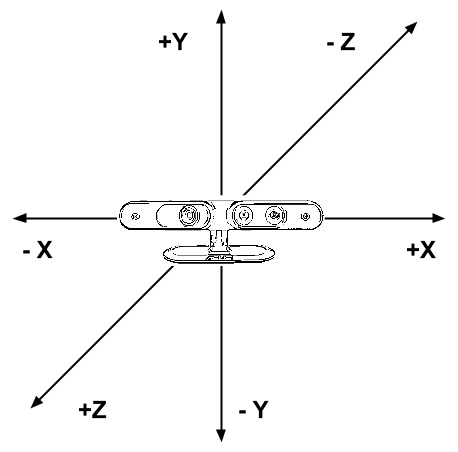
\includegraphics[height=6cm]{figures/content/xtion-origin.jpg} \caption{Depth Camera origin} \label{fg:xtion:origin} 
\end{figure}


Brain is set to training mode and CC is started to visualize the hand positions in order to align the trainer during the preparation time. Each gesture is isolated in time and gesticulated for 20 seconds. Samples are added to the training dataset and when the timer stopped the recording, Brain asked the trainer to train the same class again or another. Every gesture was assigned a class label from 1 to 5 and the mapping of class label to hand gesture is stored in a configuration file named signs.json. 

\begin{figure}
	[h] \centering 
	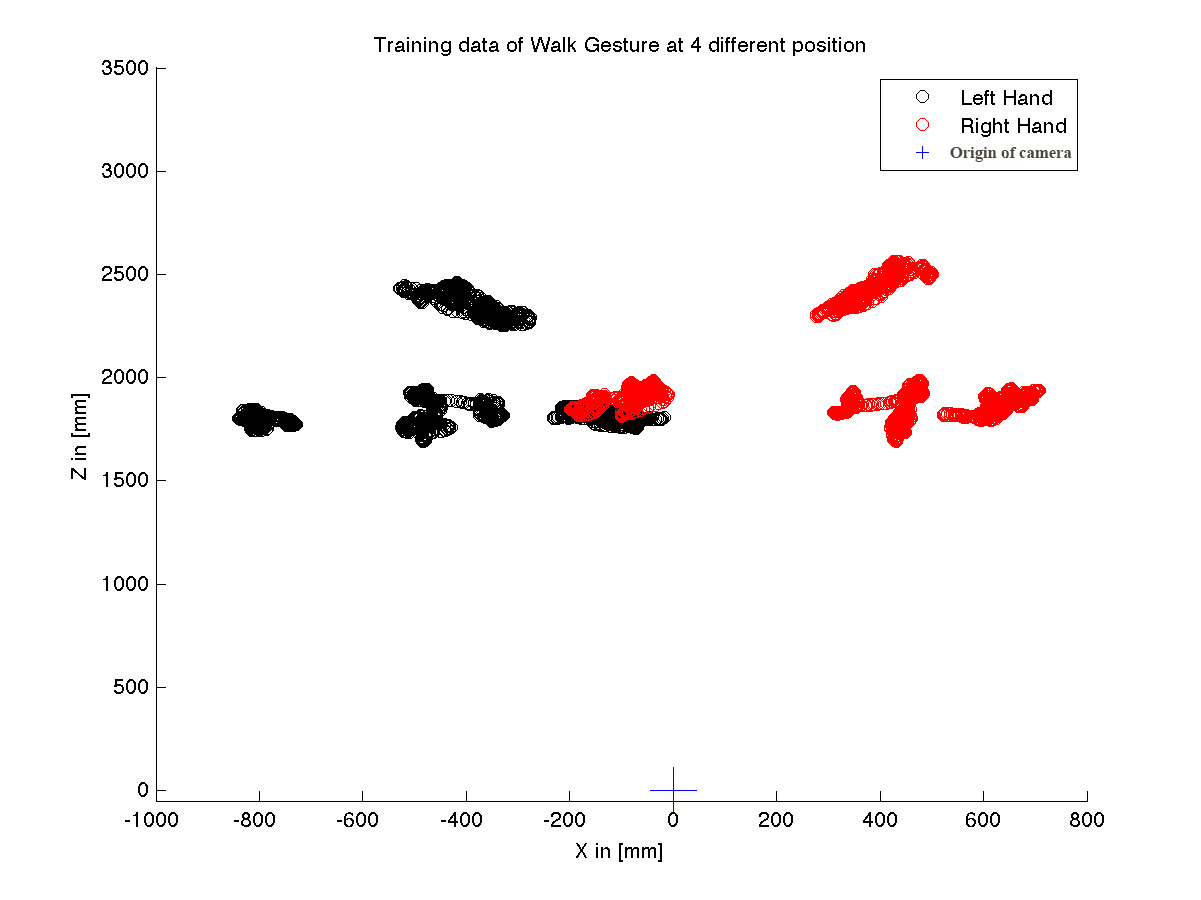
\includegraphics[height=10cm]{/result/train-walk-all.jpg} \caption{Training data of walk gesture recorded in 4 different positions with the minimum distance from 1700 mm to the maximum distance 2500 mm away from the sensor and 800 mm left or right to the origin of the depth camera.} 
	\label{fg:ges:pos} 
\end{figure}


\paragraph*{Minimum and Maximum Distance Training} \label{sec:range:train} If the gestures are gesticulated with only one person at a static position in space in front of the camera, then the recognition algorithm would not recognize the same gesture gesticulated by another person or the same person in different position. In order to scale the range of recognition, every gesture was gesticulated in 4 different positions as shown in the plot \ref{pl:ges:pos} and in all possible combinations that hands are kept wider or narrower as shown in the plots \ref{fg:ges:plot}. Therefore, each gesture in the training data is recorded in 4 positions with each for 20 seconds at 30 samples per second created 2400 samples per gesture. 

ANBC is an iterative learning algorithm that improves the classification accuracy with increase in positive training data. Plot \ref{fg:ges:plot} shows that the trained data makes our gesture recognition system to detect gestures at the minimum distance from 1700 mm to the maximum distance 2500 mm away from the sensor and 800 mm left or right to the sensor. If the user leaves this field of view, the hand tracking algorithm will lose the hand or gesture will fall in the Null Rejection region of the classifier.

\begin{figure}	 	
	\begin{minipage}
		{.45 
		\textwidth}  
		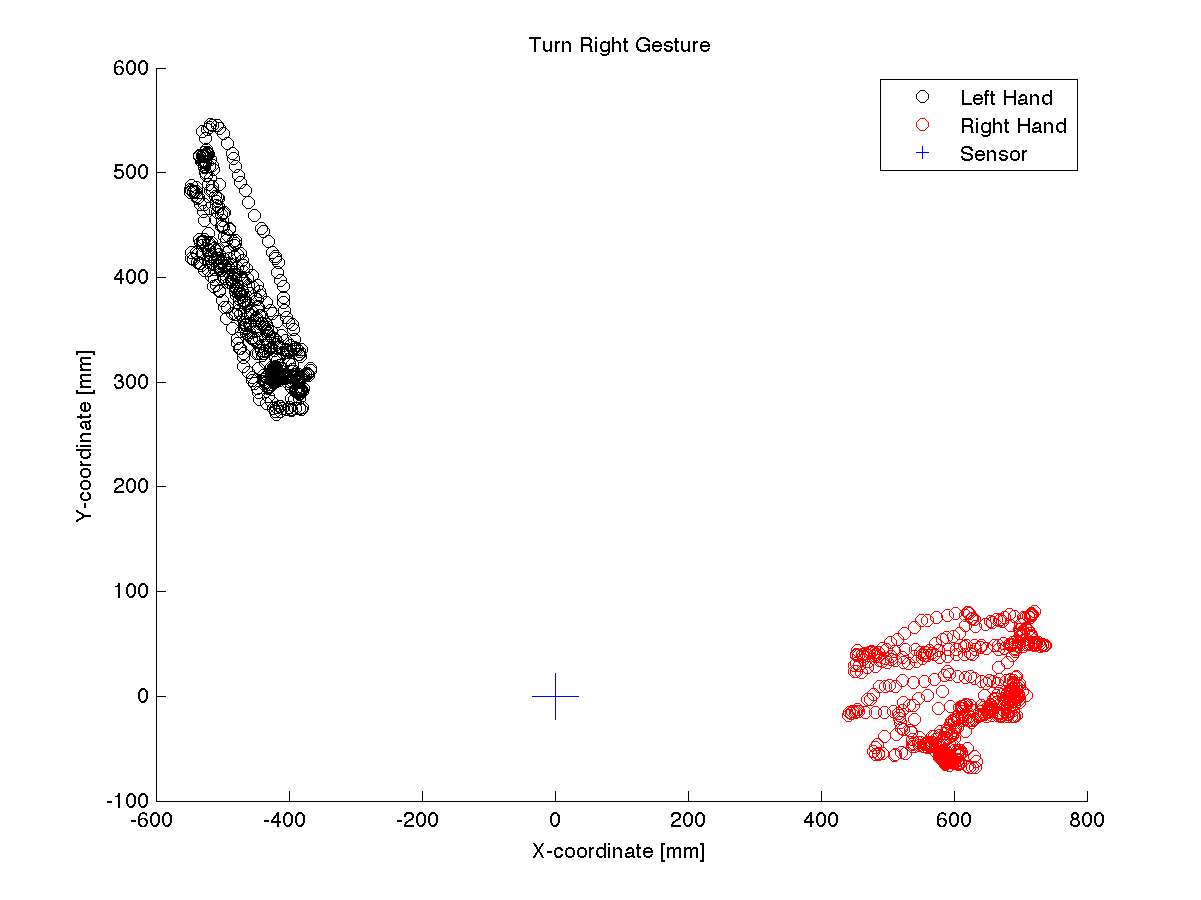
\includegraphics[height=60mm]{figures/result/plot-ges-2.png} \caption{Turn Left Gesture} \label{pl:ges:2} 
	\end{minipage}
	\begin{minipage}
		{.45 
		\textwidth}  
		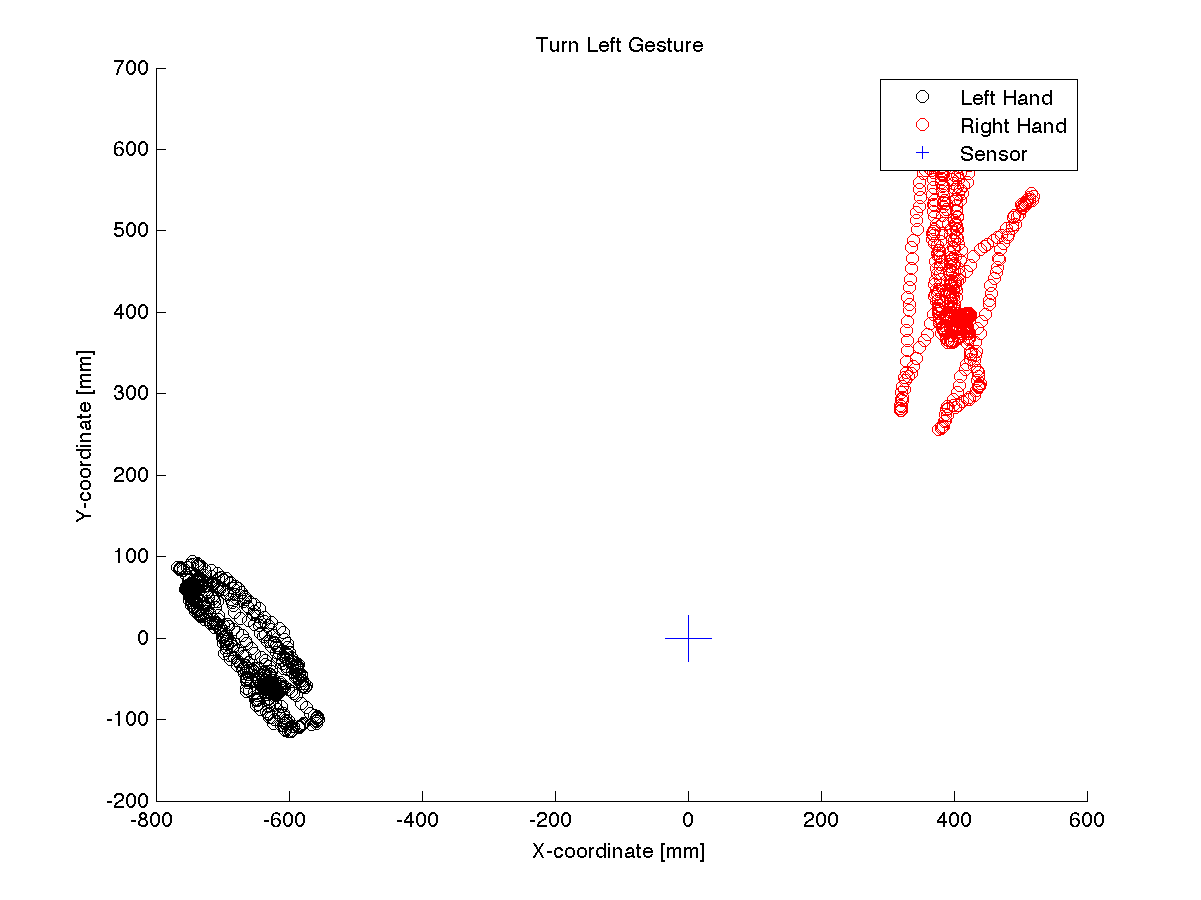
\includegraphics[height=60mm]{figures/result/plot-ges-3.png} \caption{Turn Right Gesture} \label{pl:ges:3} 
	\end{minipage}
	\begin{minipage}
		{.45 
		\textwidth}  
		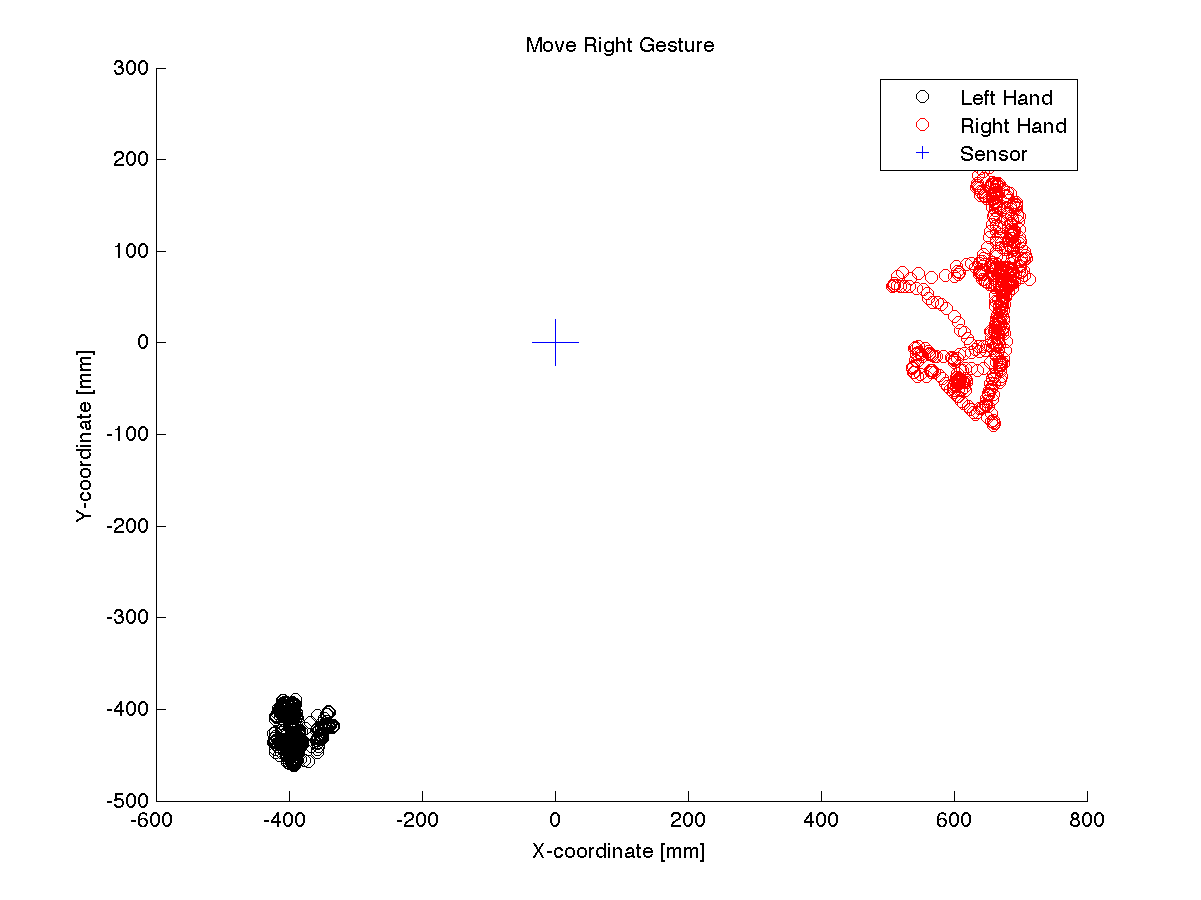
\includegraphics[height=60mm]{figures/result/plot-ges-4.png} \caption{Move Left Gesture} \label{pl:ges:4} 
	\end{minipage}
	\begin{minipage}
		{.45 
		\textwidth}  
		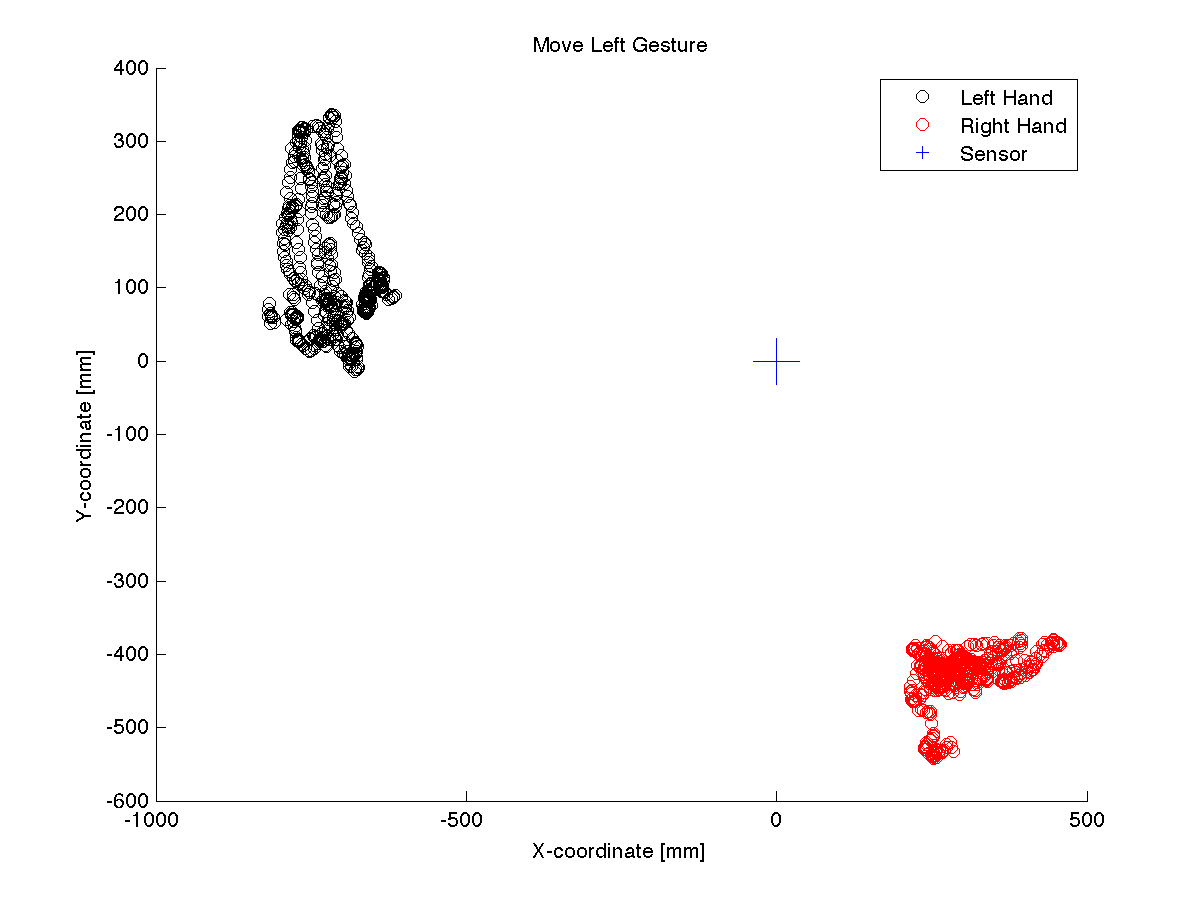
\includegraphics[height=60mm]{figures/result/plot-ges-5.png} \caption{Move Right Gesture} \label{pl:ges:5} 
	\end{minipage}
	\begin{minipage}
		{.45 
		\textwidth}  
		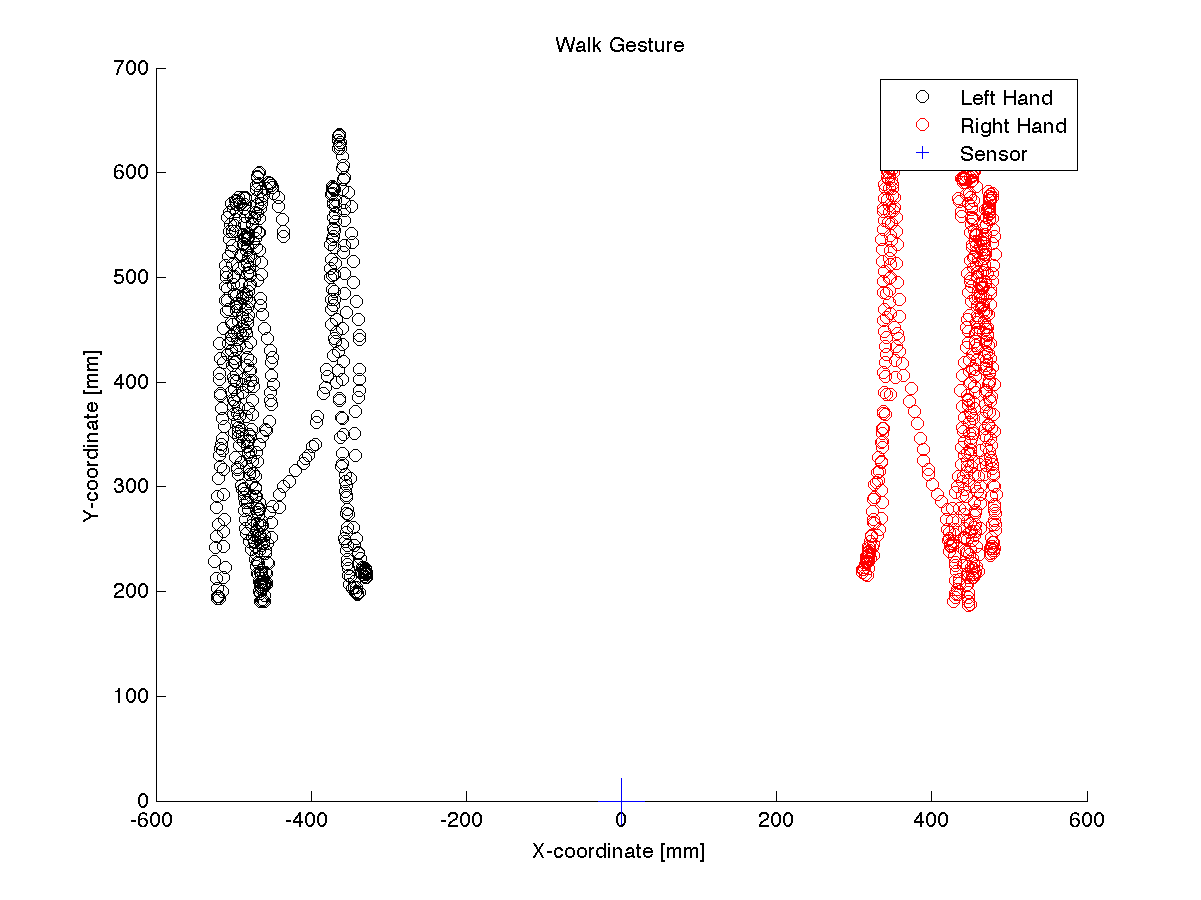
\includegraphics[height=60mm]{figures/result/plot-ges-1.png} \caption{Walk Gesture} \label{pl:ges:1} 
	\end{minipage}	
\end{figure}
\label{fg:ges:hands} \label{fg:ges:plot}



\paragraph*{Training Data} Once all the gestures are recorded, they replayed using CC to find out, if there is any false samples are added to the training data. Such false data leads to an incorrect model that will ultimately affect the prediction performance. Such samples are removed from the training data and a final dataset with all 5 classes are stored as hri-training-dataset.txt. Additionally, some test data for each gesture is recorded in order to evaluation the accuracy of the recognition system. Furthermore, a set of non-gesture dataset was recorded in order to test the Null Rejection accuracy of the classifier. 

\subsection{Prediction} After successfully collecting the training data for all the gestures, Brain is set to prediction mode where the pipeline is trained. HRI module starts to track the user's hand, Brain predicts a gesture when both the hands are present in the input sample. Figure \ref{fg:cc:walk} shows Control Center where prediction output for every sample with maximum likelihood is displayed all the time. The predicted gesture is triggered only after it was gesticulated for more than one second.

\begin{figure}
	[h] \centering 
	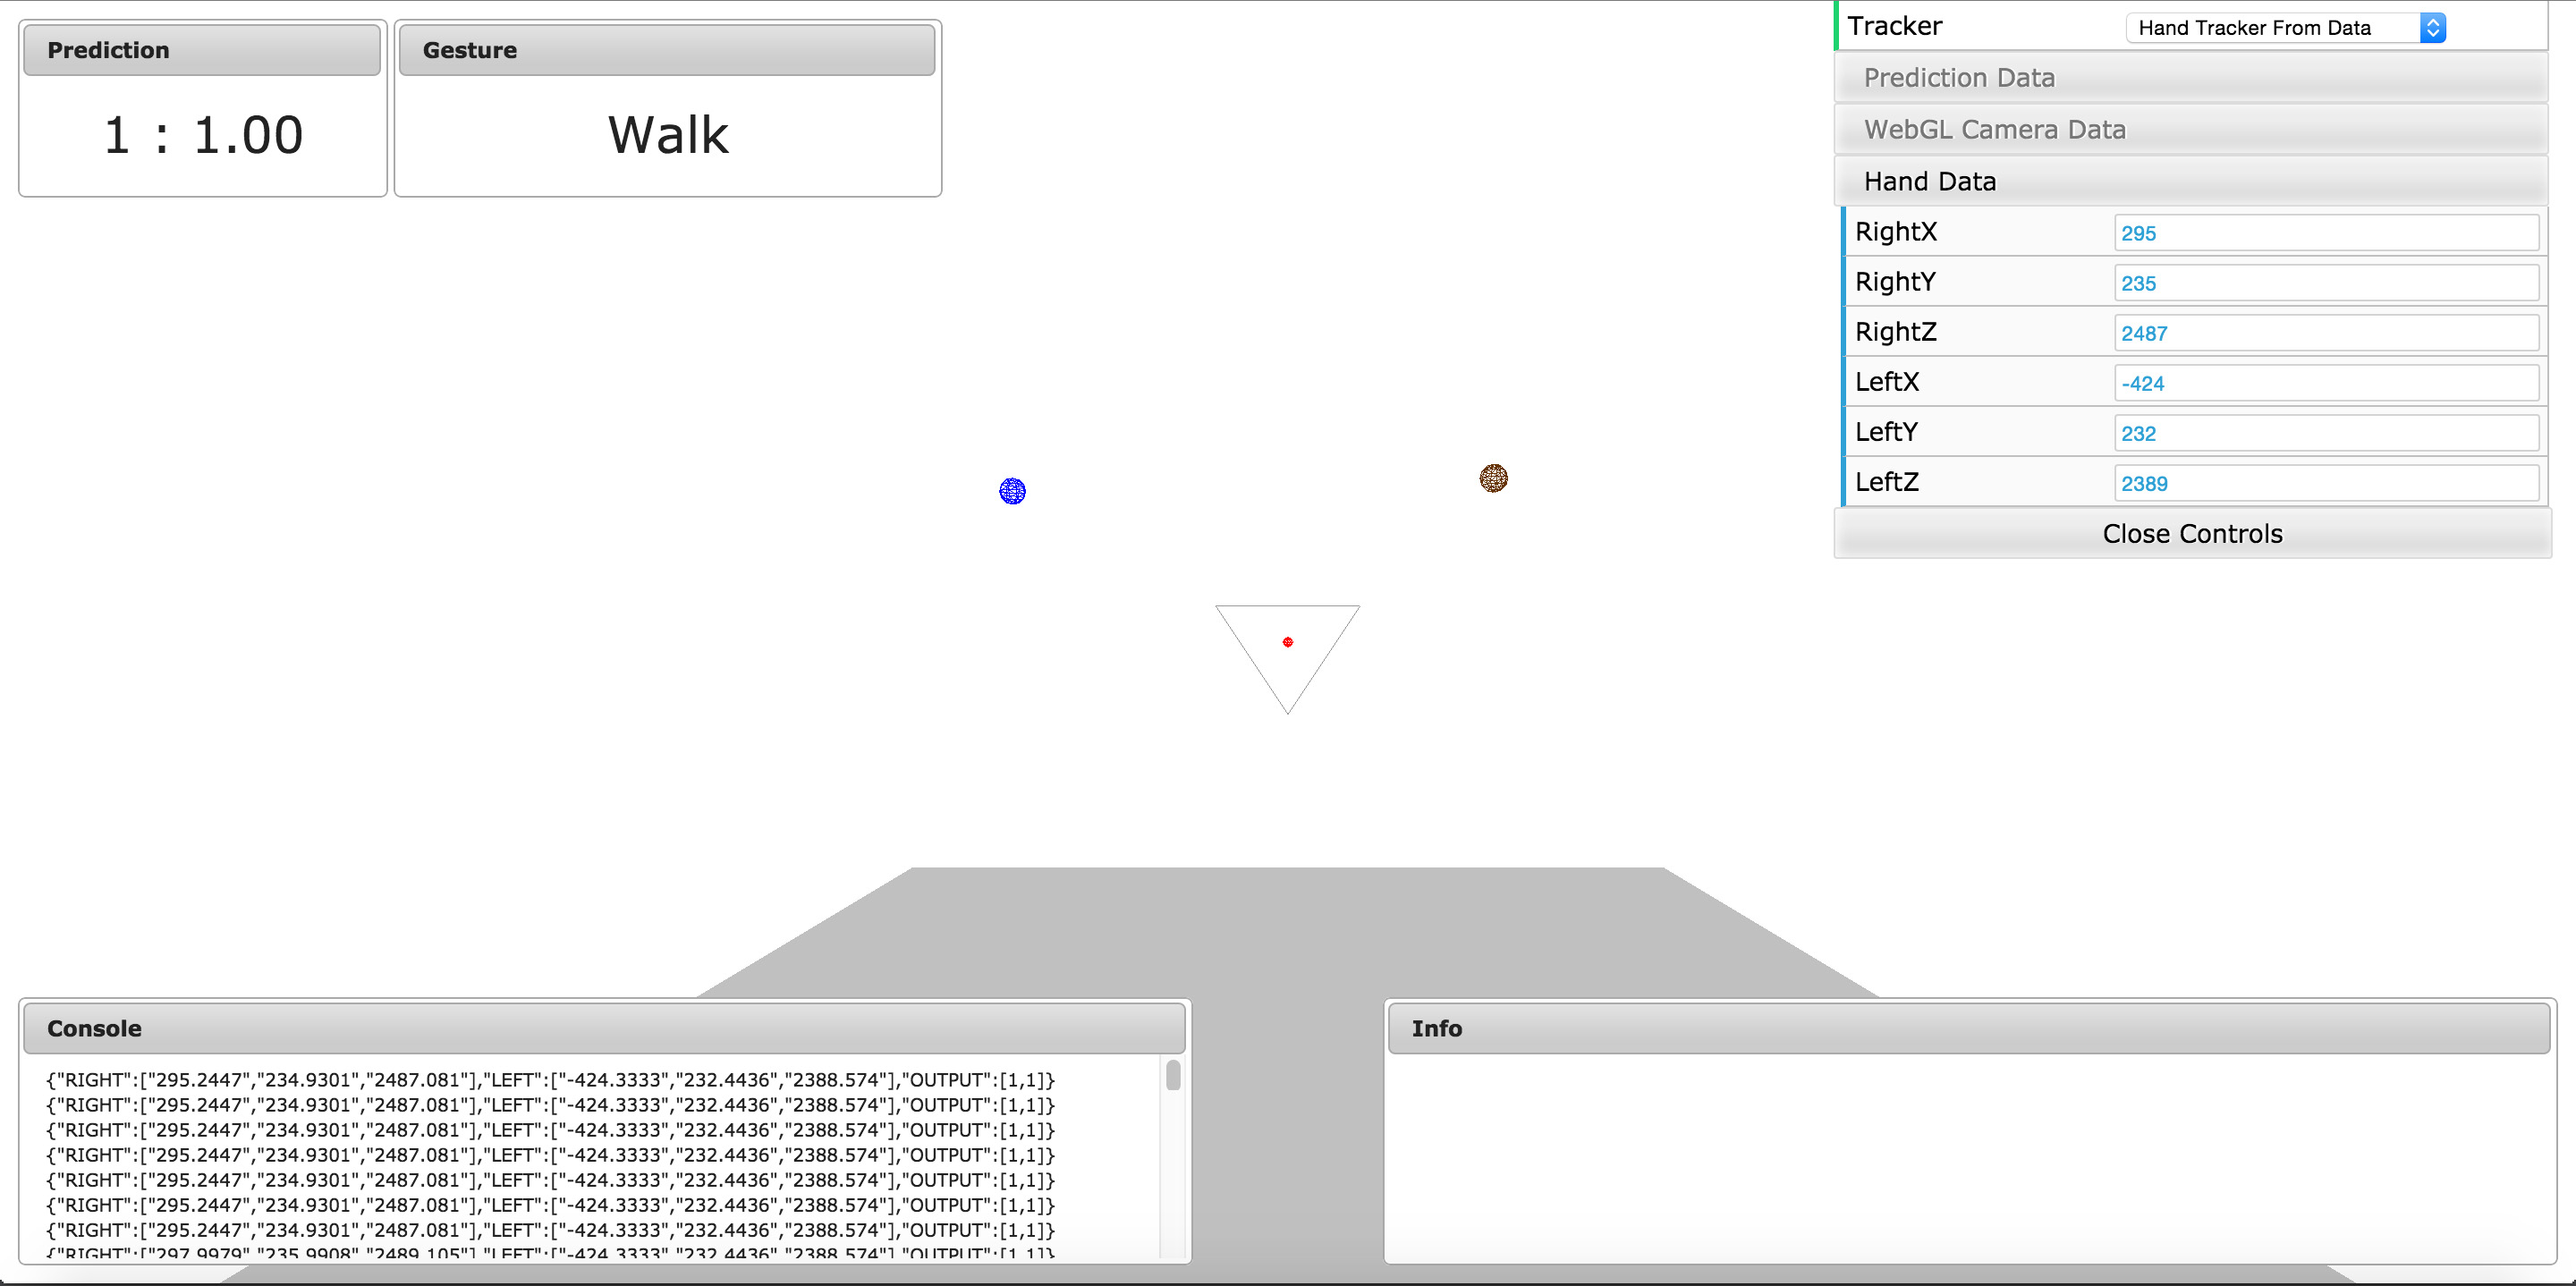
\includegraphics[width=125mm]{figures/result/cc-walk.jpg} \caption{Control Center displays the recognized walk gesture in real time with the positions of left and right hand in 3 dimensional space. } \label{fg:cc:walk} 
\end{figure}

